\documentclass[12pt]{article}
\usepackage{latexsym}
\usepackage{tikz} 
\usepackage{epsfig}

\setlength{\topmargin}{0in}
\setlength{\leftmargin}{0in}
\setlength{\textwidth}{6in}
\setlength{\textheight}{9.5in}
\setlength{\parindent}{0.2in}
\setlength{\parskip}{.08in}
\voffset = -.45in
\hoffset = -.5in
\def\filledbox{\vrule height 1.8ex width .8ex depth -.1ex }
% square bullet
\newcommand{\qed}{\large ~$\Box$ \normalsize}
%
%\newtheorem{thm}{Theorem}
%\newenvironment{theorem}{\begin{thm}\ \rm}{\end{thm}}
%
%\newtheorem{lem}{Lemma}
%\newenvironment{lemma}{\begin{lem}\ \rm}{\end{lem}}
%
\newtheorem{theorem}{Theorem}
\newtheorem{lemma}{Lemma}
\newtheorem{corollary}{Corollary}
\newenvironment{proof}{{\noindent \bf Proof\ \ }}{\qed}
\newenvironment{proofsketch}{{\noindent {\bf Proof}\ (sketch)\ \ }}{\qed}
%
\def\shh{\skew3\hat{\hat s}}
\def\dhh{\skew6\hat{\hat d}}
\begin{document}
\newcommand{\I}{\mbox{{\em Int}}}
\newcommand{\lt}{\mbox{{\em left}}}
\newcommand{\rt}{\mbox{{\em right}}}
\newcommand{\ld}{\Delta^l}
\newcommand{\rd}{\Delta^r}
\newcommand{\lsp}[1]{\large\renewcommand{\baselinestretch}{#1}\normalsize}
\newcommand{\hsp}{\hspace{.2in}}

\def\Endwhile{\mbox{\bf endwhile\ }}
\def\Or{\mbox{\bf or\ }}
\def\Do{\mbox{\bf do\ }}
\def\Downto{\mbox{\bf downto\ }}
\def\Int{\mbox{\bf int\ }}
\def\To{\mbox{\bf to\ }}
\def\Repeat{\mbox{\bf repeat\ }}
\def\Until{\mbox{\bf until\ }}
\def\Return{\mbox{\bf return\ }}
\def\Not{\mbox{\bf not\ }}
\def\And{\mbox{\bf and\ }}
\def\For{\mbox{\bf for\ }}
\def\Foreach{\mbox{\bf foreach\ }}
\def\Else{\mbox{\bf else\ }}
\def\Elseif{\mbox{\bf elseif\ }}
\def\End{\mbox{\bf end\ }}
\def\If{\mbox{\bf if\ }}
\def\Mod{\mbox{\bf \ mod\ }}
\def\Then{\mbox{\bf then\ }}
\def\While{\mbox{\bf while\ }}
\def\Output{\mbox{\bf output\ }}

\lsp{1}
\pagestyle{plain}
\begin{center}
    {\bf
        Flow/Residual Network Worksheet
    }
\end{center}

The table below shows the capacity and flow for each directed edge in a
flow network with source 0 and sink 5.

\begin{table}[h]
    \center
    \begin{tabular}{|c|c|c|} \hline
        Directed edge & capacity & flow \\ \hline
        (0,1)         & 2        & 2    \\
        (0,2)         & 3        & 1    \\
        (1,3)         & 3        & 2    \\
        (1,4)         & 1        & 0    \\
        (2,3)         & 1        & 0    \\
        (2,4)         & 1        & 1    \\
        (3,5)         & 2        & 2    \\
        (4,5)         & 3        & 1    \\ \hline
    \end{tabular}
\end{table}

\begin{enumerate}
    \item Draw the flow network.\\
    The fractions represent flow over capacity.
    \begin{center}
        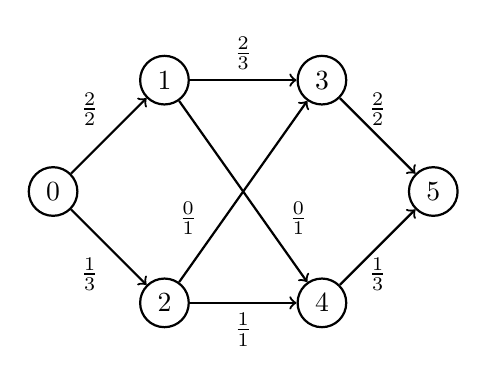
\begin{tikzpicture}[node distance={2cm}, thick, main/.style = {draw, circle}] 
            \node[main] (0) {0};
            \node[main] (1) [above right of=0]{1};
            \node[main] (2) [below right of=0] {2};
            \node[main] (3) [right of=1] {3};
            \node[main] (4) [right of=2] {4};
            \node[main] (5) [above right of=4] {5};
    
            % tree edges
            \draw[->] (0) -- (1) node [midway,above left] {$\frac{2}{2}$}; 
            \draw[->] (0) -- (2) node [midway,below left] {$\frac{1}{3}$}; 
            \draw[->] (1) -- (3) node [midway,above] {$\frac{2}{3}$}; 
            \draw[->] (1) -- (4) node [midway,below,xshift=7mm] {$\frac{0}{1}$}; 
            \draw[->] (2) -- (3) node [midway,below,xshift=-7mm] {$\frac{0}{1}$}; 
            \draw[->] (2) -- (4) node [midway,below] {$\frac{1}{1}$}; 
            \draw[->] (3) -- (5) node [midway,above] {$\frac{2}{2}$}; 
            \draw[->] (4) -- (5) node [midway,below] {$\frac{1}{3}$}; 
        \end{tikzpicture}
    \end{center}
    \item Draw the residual network.
    \begin{center}
        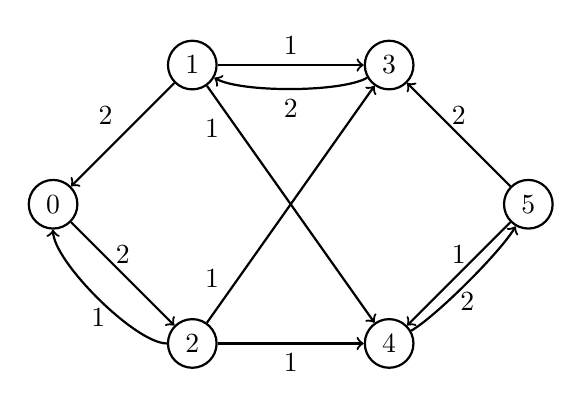
\begin{tikzpicture}[node distance={2.5cm}, thick, main/.style = {draw, circle}] 
            \node[main] (0) {0};
            \node[main] (1) [above right of=0]{1};
            \node[main] (2) [below right of=0] {2};
            \node[main] (3) [right of=1] {3};
            \node[main] (4) [right of=2] {4};
            \node[main] (5) [above right of=4] {5};
    
            % tree edges
            \draw[->] (1) -- (0) node [midway, above left] {2};
            \draw[->] (0) -- (2) node [midway, above] {2};
            \draw[->] (2) to [out=180, in=270, looseness=.5] node [midway, below] {1} (0);
            \draw[->] (1) -- (3) node [midway, above] {1};
            \draw[->] (3) to [out=210, in=330, looseness=.5] node [midway, below] {2} (1);
            \draw[->] (1) -- (4) node [midway, below,xshift=-10mm,yshift=12mm] {1};
            \draw[->] (2) -- (4) node [midway, below] {1};
            \draw[->] (2) -- (3) node [midway, below,xshift=-10mm,yshift=-7mm] {1};
            \draw[->] (5) -- (3) node [midway, above] {2};
            \draw[->] (5) -- (4) node [midway, above] {1};
            \draw[->] (4) to [out=30, in=240, looseness=.5] node [midway, below] {2} (5);
        \end{tikzpicture}
    \end{center}

    \item Identify an augmenting path from the source to the sink in the
          residual network.

          $0 \to 2 \to 3 \to 1 \to 4 \to 5$
\end{enumerate}

\end{document}